\chapter{Arquitectura}
\label{cap:arquitectura}

\section{Análisis de los recuerdos}

Los sistemas de análisis automático de texto tienen como objetivo entender la información no estructurada hablada por los humanos y convertirla en información estructurada como podría ser un resumen del contenido o la clasificación de un documento por temática. En este caso, se busca conseguir esta información estructurada a partir de la mayor cantidad de recuerdos posibles para ayudar a los terapeutas a construir la historia de vida de un paciente que es mucho más complicada de tratar en bruto. El análisis que se pretende realizar de estos recuerdos es por un lado clasifican en etapas de vida. El análisis se va a realizar en varios sentidos, por un lado, se clasificarán los recuerdos en etapas de vida, para estructurar la información lo máximo posible. Por otro lado, se determinará si el texto contiene connotaciones positivas o negativas, de tal forma que en la terapia se puedan evitar los recuerdos negativos que pueden agravar la situación del paciente. Por último, se utilizará el procesamiento del lenguaje natural mediante el análisis morfológico de las palabras para comprender lo que quiere decir el paciente y poder generar la respuesta más acertada y relacionada con la temática que se está tratando. 

\subsection{Clasificación de los recuerdos}

Se ha probado una forma de clasificar texto utilizando TextCategorizer \footnote{https://spacy.io/api/textcategorizer} de la librería spacy de python. Se trata de entrenar un modelo para saber identificar si un recuerdo es positivo o negativo. Se ha utilizado el código del artículo \textit{How to Train Text Classification Model in spaCy} \footnote{https://www.machinelearningplus.com/nlp/custom-text-classification-spacy/} para probar cómo se podría entrenar el modelo para que supiese diferenciar los recuerdos negativos de los positivos y así tener la primera clasificación que pidieron los terapeutas especializados del proyecto CANTOR. Antes de probar con recuerdos se probó con un dataset muy grande de reseñas de moda que se ponía como ejemplo en el artículo del que hablábamos anteriormente. Después, se ha probado usando una batería menor de recuerdos positivos encontrados entre los archivos del TFG de Laura Castillo \citep{reminiscencia}. También había que incluir recuerdos negativos, como no se ha encontrado ningún dataset ni textos relacionados, se han usado frases negativas aleatorias.

El prototipo funciona siguiendo una serie de pasos. En primer lugar, se añade el componente TextCategorizer (textcat) a un modelo en blanco del idioma español. Un modelo en blanco es un modelo que no tiene ningún componente de spaCy definido (como serían NER que explicaré más adelante), es decir, el texto que se almacena en los documentos de spaCy no es analizado por ninguna cadena de procesos porque la tubería de componentes está vacía. Si hubiésemos cogido un modelo pre-entrenado como ``es\_core\_news\_sm'', el clasificador de textos se sumaría al trabajo previo de los procesos que analizan el texto como serían ['tok2vec', 'morphologizer', 'parser', 'attribute\_ruler', 'lemmatizer', 'ner']. Por ejemplo, el componente NER, más reconocido como \textit{Named Entity Recognizer}, reconoce entidades dentro del texto como nombres de personas, fechas o lugares. Al usar el modelo en blanco empezamos con el español de cero, sin analizar. Tras añadir el componente textcat, al crear un documento de spaCy, automáticamente, pasará por el proceso de clasificación que le indiquemos. Para que textcat funcione como categorizador de recuerdos, se le añade a nuestro nuevo componente dos etiquetas, NEGATIVO y POSITIVO, que definirán cuánto de negativo es un recuerdo y cuánto de positivo. Para seguir configurándolo, el prototipo coge el texto que usaremos para entrenar nuestro modelo y lo prepara adecuándolo al formato que entiende el clasificador, siendo éste una lista de tuplas (texto, etiqueta). Además, cogerá un porcentaje de esta batería de recuerdos (\% que previamente hemos definido) y lo reservará para la evaluación de las predicciones, es decir, para analizar cómo de bien predice nuestro modelo tras entrenarlo. 

Ya tenemos casi todo preparado para comenzar a entrenar el modelo, se dividen los casos de entrenamiento en lotes que se analizarán y evaluarán un número definido de iteraciones para asegurar que el entrenamiento es lo más preciso posible sin pasarnos de vueltas para que sea óptimo. Se trata de un proceso iterativo en el que las predicciones del modelo se comparan con las etiquetas de referencia para estimar el gradiente de la pérdida. El modelo se entrena utilizando una función que lo analiza y actualiza en cada iteración, la función update(). También se comprueban las predicciones del modelo en cada vuelta, se comparan con las etiquetas de referencia para estimar la desviación de la pérdida.

Una vez afinado el modelo mediante el entreno previo, ya podemos ponerlo a prueba. El prototipo sacará la probabilidad de que un texto procesado por spacy sea un recuerdo positivo y la probabilidad de que sea uno negativo. 

--------Meter problemas probando el neutro

\subsubsection{Análisis de sentimiento}

\subsubsection{Clasificación en etapas de vida}

Para categorizar las respuestas según el sentimiento usaremos directamente el prototipo del apartado de análisis de sentimientos de un texto. Se ha añadido un archivo ``analyze\_answer'' que entrena primero al modelo con textos positivos y negativos y luego evalúa el texto que le llega e identifica si es negativo o positivo. Esto se añade como una categoría que se meterá en la base de datos junto a la respuesta. Este análisis de sentimiento también servirá para identificar temáticas dolorosas para el interrogado que no deberían ser usadas en las terapias. 

Otra categoría que se añadirá junto a la respuesta será la de la etapa de la vida a la que corresponde. Primero tenemos que definir esas etapas y para ello me he basado en la clasificación que hace el Ministerio de Salud de Colombia ( https://www.minsalud.gov.co/proteccionsocial/Paginas/cicloVida.aspx) porque no he encontrado ninguna clasificación tan clara para España y me parecía una forma sensata de clasificación. Le he hecho algunas modificaciones para adecuarme más a lo que quería sacar en claro de la información que se me presentaba. Las etapas serían las siguientes:
\begin{itemize}
	\item Infancia de 0 a 11 años
	\item Adolescencia de 12 a 17 años
	\item Juventud de 18 a 26 años
	\item Etapa adulta de 27 a 59 años
	\item Vejez de 60 años o más
	\item Indeterminado para aquellos textos en los que no se pueda distinguir la etapa
\end{itemize}

Una vez elegidos los periodos de tiempo en los que se divide la vida de las personas, el objetivo es clasificar recuerdos, dados en forma de respuesta a una pregunta, según la etapa de la vida a la que pertenecía el recuerdo de la persona interrogada. Para ello, también se ha utilizado la misma tecnología que el prototipo primero de análisis de sentimientos. Además de entrenarse en recuerdos positivos y negativos, ahora el modelo se entrena para distinguir etapas vitales en las que ocurren los recuerdos para así, de cara a la elaboración de un libro de vida, que toda la información esté bien estructurada en periodos de tiempo. 

---- Meter problemas con la etapa de vida indeterminada 

Se ha probado con neutro pero no funcionaba igual de bien, se necesitan muchos más textos de entrada. Para poder hacer este análisis se han utilizado los recursos de la una pagina web \footnote{https://www.machinelearningplus.com/nlp/custom-text-classification-spacy/} de demostración del uso de spacy. El manual de usuario de spacy \footnote{https://spacy.io/api/textcategorizer} no ha resultado ser muy explicativo.

\subsection{Procesamiento del texto para encadenar preguntas y respuestas}
 
Esta sección consiste en conseguir que las preguntas que se hagan al interrogado tengan sentido con el resto de la conversación previa. Conseguir que sean lo más inteligentes y adecuadas posible. 

Lo primero que se ha hecho para encontrar la siguiente pregunta a hacer es coger la lista de todas las posibles preguntas y eliminar aquellas que ya han sido contestadas anteriormente para no repetirlas. 

Lo siguiente que se hará es pasar tanto la respuesta más reciente que ha dado el interrogado como todas las posibles preguntas por un proceso de síntesis. Para ello vamos a utilizar el analizador de texto Spacy utilizando el código del TFG de Laura Castilla Castellano (Generación de historias a partir de una base de conocimiento), en concreto el código que aparece en el archivo ``analysis.py'' de su código, que contiene funciones para el procesamiento y síntesis de los textos. Los pasos que Laura sigue para el análisis del texto aparecen en el apartado 5.1 (Analizar textos para obtener sugerencias) de su memoria, páginas 30 y 31. Las funciones que se han reutilizado en este trabajo, con algunas modificaciones, son las siguientes:
\begin{itemize}
	\item Read: Coge el texto a analizar y elimina signos de puntuación
	\item Synthesis: Elimina las palabras vacías como las preposiciones del texto
	\item Lemmatize: Transforma cada palabra del texto sus lemas correspondientes
	\item Categorize: Separa las palabras en sustantivos, verbos y adjetivos. Además, coge los 30 más comunes de cada tipo
	\item Get\_most\_common\_words: Coge las palabras más comunes de todos los tipos del texto
\end{itemize}

Estas funciones se han utilizado para conseguir una representación del texto más precisa y reducida. Solo los lemas de las palabras importantes del texto serán usados para este módulo de encadenamiento de preguntas y respuestas.

Por último, dada la respuesta y todas las posibles preguntas ya reducidas a sus lemas, para encontrar la pregunta más adecuada, se compara una a una los lemas de las posibles preguntas con los lemas de la respuesta. Dentro de la lista de posibles preguntas, la que más lemas comunes tenga con la respuesta, gana como siguiente pregunta a formular.


\section{Bases de datos}

Se han usado dos tipos de bases de datos, una relacional en MySQL encargada de almacenar datos de inicio de sesión para la página web del chatbot. La otra base de datos es no relacional levantada en MongoDB que almacena los datos relacionados con los recuerdos de la persona con demencia y de la interacción con el chatbot. 

\subsection{MySQL}

Se trata de una base de datos ideal para conjuntos de datos que tienen una estructura fija, como en este caso, los datos de inicio de sesión de los usuarios y los datos de las terapias que asocian a los terapeutas con sus pacientes. Es por esto que se ha construido una base de datos con dos tablas, una que identifica a los usuarios y otra que guarda la información sobre las terapias. En la figura \ref{fig:diseñoinicialappterapeuta1}

\begin{figure}[h]
	\centering
	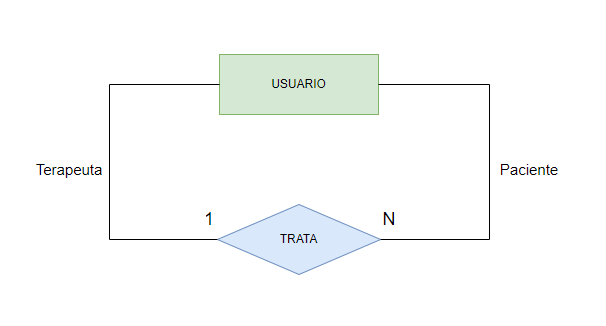
\includegraphics[scale=1.0]{Imagenes/Vectorial/diagrama_entidad_relacion_mysql}
	\caption{Diagrama de entidad-relación MySQL}
	\label{fig:diagramaEER}
\end{figure}

\subsubsection{Tabla de usuarios}
de usuarios en la que para cada registro tendremos el identificador, único y clave primaria; el nombre de usuario; el correo electrónico, único también, y la contraseña, que se guardará cifrada. Cuando se intente iniciar sesión, se comprobará si los datos son correctos.

\begin{figure}[h]
	\centering
	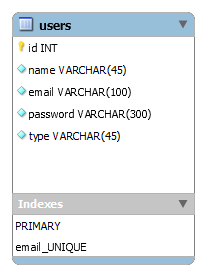
\includegraphics[scale=1.0]{Imagenes/Vectorial/diagrama_tabla_users}
	\caption{Diagrama de la tabla de usuarios}
	\label{fig:diagramatablausers}
\end{figure}

\begin{figure}[h]
	\centering
	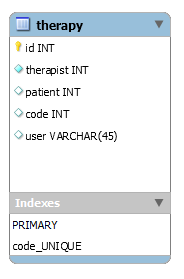
\includegraphics[scale=1.0]{Imagenes/Vectorial/diagrama_tabla_therapy}
	\caption{Diagrama de la tabla de terapias}
	\label{fig:diagramatablatherapy}
\end{figure}


\subsection{MongoDB}



\section{Aplicación web}

La aplicación web se ha creado con el objetivo de proporcionar funcionalidades tanto para los posibles terapeutas como para sus posibles pacientes. Por un lado, el chatbot se ha pensado para que lo usen los pacientes y es el foco principal de este TFG y, donde se han aplicado todas las técnicas que se han tratado en las secciones anteriores. La aplicación web permite probar el chatbot de forma mucho más manejable y visible que desde un terminal del entorno de desarrollo. Por otro lado, se ha querido añadir las funcionalidades para los supuestos terapeutas que, podrían acceder a los recuerdos de sus pacientes de forma sencilla y visual.

\subsection{Prototipo inicial}

Al inicio de este trabajo, había que ver qué dirección se iba a seguir, en esos momentos yo planteaba a mis tutores diferentes ideas que se me iban ocurriendo y ellos me guiaban por la propuesta más adecuada. Una de las ideas que se propusieron era la de este prototipo de aplicación web inicial. Realicé un esbozo sobre lo que creía que iba a necesitar el chatbot como aplicación para estar completo. Este prototipo a mano alzada está dividido en dos partes. Por un lado, están las funcionalidades pensadas para el uso del terapeuta, que podrá programar las sesiones que quiere hacer personalmente con el paciente (ver Figuras \ref{fig:diseñoinicialappterapeuta1}, \ref{fig:diseñoinicialappterapeuta2}, \ref{fig:diseñoinicialappterapeuta3}, \ref{fig:diseñoinicialappterapeuta4}, \ref{fig:diseñoinicialappterapeuta5}). Por otro lado, están las funcionalidades pensadas para el paciente con demencia (ver Figura \ref{fig:diseñoinicialappusuario}) y que hará uso del chatbot en sí. Es importante aclarar que el terapeuta tiene sus sesiones con el paciente como se hace habitualmente y las funcionalidades que tiene disponibles en la aplicación son para ayudarle a programar esas sesiones. El chatbot es solo accesible desde la cuenta de un paciente porque es una herramienta de apoyo para el terapeuta para facilitar la recolección de recuerdos del paciente y, conseguir la información de otra forma para así ganar tiempo.

Para el usuario con demencia el prototipo es muy sencillo, tiene 2 funcionalidades básicas propias (ver Figura \ref{fig:diseñoinicialappusuario}):

\begin{figure}[h]
	\centering
	\includegraphics[scale=1.0]{Imagenes/Vectorial/diseño app tfg 2}
	\caption{Prototipo inicial de la aplicación para el usuario con demencia}
	\label{fig:diseñoinicialappusuario}
\end{figure}

\begin{itemize}
	\item Chatbot: La pestaña de terapia lleva al usuario al chat donde se le hará preguntas sobre su vida para recabar el máximo número de recuerdos. El chatbot es un complemento aparte que ayuda al terapeuta a recoger la información del usuario pero que no sustituye las sesiones habituales paciente-terapeuta.
	\item Historia de vida: Los recuerdos recabados se guardan en la aplicación y el usuario puede consultarlos divididos por etapas de la vida (infancia, adolescencia, etapa adulta, etc.). Esto sería parte de la terapia ocupacional basada en reminiscencia y un paso previo para construir el libro de vida del usuario. El usuario puede revisitar sus recuerdos a través de la aplicación y esto puede ayudar en el retraso del deterioro cognitivo.
\end{itemize}

En cuanto a las vistas del terapeuta, tendrá muchas más funcionalidades disponibles:

\begin{figure}[h]
	\centering
	\includegraphics[scale=0.1]{Imagenes/Vectorial/diseño app tfg 1-1}
	\caption{Prototipo inicial de la aplicación para el terapeuta: Consultar los pacientes registrados}
	\label{fig:diseñoinicialappterapeuta1}
\end{figure}

Ver Figura \ref{fig:diseñoinicialappterapeuta1} $\rightarrow$
\begin{itemize}
	\item Pacientes: Se muestra una lista de los usuarios (pacientes) que tiene el terapeuta asignados y que están registrados en la aplicación. 
\end{itemize}

\begin{figure}[h]
	\centering
	\includegraphics[scale=0.1]{Imagenes/Vectorial/diseño app tfg 1-2}
	\caption{Prototipo inicial de la aplicación para el terapeuta: Consultar los datos de un paciente 1}
	\label{fig:diseñoinicialappterapeuta2}
\end{figure}

Ver Figura \ref{fig:diseñoinicialappterapeuta2} $\rightarrow$
\begin{itemize}
	\item Datos personales del paciente: Los datos personales y clínicos del paciente estarán disponibles para que el terapeuta los consulte cuando quiera.
	\item Terapias del paciente: Se muestran las terapias que se han creado para ese paciente, tanto las que se programaron para fechas pasadas como las que ocurrirán próximamente. El terapeuta es el que crea estas terapias para sus futuras sesiones con el paciente, las terapias pasadas son las sesiones que se han finalizado y las próximas son las que están pendientes por hacer.
\end{itemize}

\begin{figure}[h]
	\centering
	\includegraphics[scale=0.1]{Imagenes/Vectorial/diseño app tfg 1-3}
	\caption{Prototipo inicial de la aplicación para el terapeuta: Consultar los datos de un paciente 2}
	\label{fig:diseñoinicialappterapeuta3}
\end{figure}

Ver Figura \ref{fig:diseñoinicialappterapeuta3} $\rightarrow$
\begin{itemize}
	\item Historia de vida del paciente: Los recuerdos recabados en las sesiones terapéuticas se guardan en la aplicación y el terapeuta puede consultarlos divididos por etapas de la vida (infancia, adolescencia, etapa adulta, etc.) igual que podía hacer el usuario. El objetivo de que el terapeuta pueda consultarlos es para revisar que se han grabado los recuerdos correctamente y para comprobar que son precisos y coherentes. En cualquier caso, el terapeuta podrá editar o borrar los recuerdos que crea incompletos o incorrectos y podrá también añadir recuerdos que haya conseguido de alguna otra forma. En caso de que algún recuerdo esté mal clasificado en la etapa de la vida en que ocurrió, también se podría mover a su sitio correcto.
\end{itemize}

\begin{figure}[h]
	\centering
	\includegraphics[scale=0.08]{Imagenes/Vectorial/diseño app tfg 1-4}
	\caption{Prototipo inicial de la aplicación para el terapeuta: Crear y consultar las terapias creadas}
	\label{fig:diseñoinicialappterapeuta4}
\end{figure}

Ver Figura \ref{fig:diseñoinicialappterapeuta4} $\rightarrow$
\begin{itemize}
	\item Terapias: Se muestra una lista ordenada de las terapias que ha ido creando el terapeuta para los distintos pacientes.
	\item Consultar terapia: El terapeuta puede revisar una terapia que haya sido ya planificada. También puede editarla o iniciar la terapia cuando esté con el paciente. 
	\item Nueva terapia: Para crear/programar una nueva terapia es necesario asignarle un nombre, el paciente al que va dirigida y una fecha en la que se llevará a cabo. El paciente se puede elegir de entre los usuarios que tiene asignados el terapeuta pero, también puede crear un nuevo usuario al que irá dirigida que no es necesario que esté registrado en la aplicación. Después, se crean por cada bloque las preguntas o temas que se quieren sacar en la sesión en el orden que quieran ser utilizados.
\end{itemize}

\begin{figure}[h]
	\centering
	\includegraphics[scale=0.1]{Imagenes/Vectorial/diseño app tfg 1-5}
	\caption{Prototipo inicial de la aplicación para el terapeuta: Consultar y reproducir una terapia concreta}
	\label{fig:diseñoinicialappterapeuta5}
\end{figure}

Ver Figura \ref{fig:diseñoinicialappterapeuta5} $\rightarrow$
\begin{itemize}
	\item Terapia finalizada: Se puede consultar una terapia que ya se ha realizado. Se podrá ver toda la información que se ha sacado, apuntes del terapeuta, la grabación de la sesión, la transcripción de la grabación, etc.
	\item Iniciar terapia: Cuando el terapeuta se reúne con el paciente para la sesión, pulsa a iniciar la terapia y obtendrá en orden los temas y preguntas que le quiere ir sacando al paciente. Podrá ir pasando de pregunta en pregunta cuando lo crea necesario. Al comenzar, puede poner a grabar la sesión para que luego se haga una transcripción automática de todo lo que ambos dicen. Esa grabación se puede pausar o continuar cuando se quiera También, se puede añadir una sección nueva que no se contemplase en la planificación pero que se quiera incluir en la terapia. Y finalmente, se puede terminar dar por finalizada la terapia pulsando en terminar. 
\end{itemize}

Este prototipo se descartó porque se centraba mucho en hacer una aplicación web y no tanto en el desarrollo de un chatbot lo suficientemente inteligente para dirigir una sesión de terapia sin necesidad del terapeuta. Con esto, no se desestima la labor del terapeuta que siempre tendría que comprobar que la información recabada por el chatbot es veraz y utilizar esa información para ayudar al usuario con una terapia cara a cara con el usuario. El chatbot es solo una herramienta de apoyo para facilitar el trabajo del terapeuta en conseguir los recuerdos de la vida del usuario. 

Por otro lado, en junio de 2022 se presetó el TFG ``Recuérdame: Aplicación de apoyo para el tratamiento de personas con problemas de memoria mediante terapias basadas en reminiscencia'', que precisamente se encarga del desarrollo de una aplicación web completa para facilitar la tarea del terapeuta que tiene que ayudar a usuarios con demencia a través de la terapia ocupacional basada en reminiscencia. Es decir, no tenía sentido que yo desarrollase una aplicación web para usuario y terapeuta porque ya se estaba desarrollando una cosa muy parecida en otro trabajo de fin de grado. Es por eso que la recomendación de mis tutores de centrarme en el desarrollo del chatbot fue la acertada. Aun así, sí que se ha desarrollado una pequeña aplicación web para mostrar de forma más visual la funcionalidad del chatbot. El diseño y la implementación de la misma se explicarán en las siguientes secciones.



\subsection{Implementación final}

---- A nivel de css no me he querido meter en detalles técnicos, porque que se vea bonito no era el objetivo principal de la aplicación sino algo secundario

Para la aplicación del chatbot, con la que el usuario con demencia interactuaría, se ha decidido usar el \textit{framework} de creación de aplicaciones ``Flask''. Se trata de un framework para la creación rápida de aplicaciones desarrolladas con Python. Se estuvo planteando usar el framework ``Django'' pero finalmente se optó por Flask porque Django es para aplicaciones mucho más grandes y complejas de lo que se proponía crear para este trabajo. Flask es mucho más intuitivo y fácil de usar, además, con solo un par de líneas se puede levantar una aplicación web sin necesidad de librerías ni herramientas accesorias. 

Para empezar con Flask, se utilizó la guía \footnote{https://flask.palletsprojects.com/en/2.2.x/quickstart/} proporcionada por la página oficial de este framework y un tutorial \footnote{https://j2logo.com/leccion-1-la-primera-aplicacion-flask/} específico para la creación de aplicaciones como esta. Para empezar con Flask lo principal es tener instalado Python e instalar las dependencias necesarias del framework. Esto se puede hacer desde el propio entorno de desarrollo elegido, en mi caso ``Visual Studio Code'', usando el instalador de paquetes ``pip'' de Python. En resumen, desde el terminal se instalaron los siguientes paquetes, necesarios para el correcto funcionamiento de la aplicación:

\begin{verbatim}
	> pip install Flask-WTF
	> pip install email-validator
	> pip install flask-login
	> pip install flask-sqlalchemy
	> pip install cryptography
\end{verbatim}

El paquete principal para que la aplicación funcione es el de Flask, en este caso Flask-WTF para que también incluya la validación de formularios, como sería el de inicio de sesión en el que se profundizará más adelante. El resto son paquetes que se han ido necesitando a lo largo del desarrollo de la aplicación para incluir ciertas funcionalidades. 

Una vez instalados los paquetes, el despliegue de la aplicación es muy sencillo y, tan solo se necesitan unas pocas líneas de código para que funcione. Lo primero sería crear un fichero python, en nuestro caso llamado ``run.py'', en el que irán los métodos asociados a las URLs que formarán la aplicación, el primer método en nuestro caso, sería el que nos lleva a la página principal, el ``index'', que es básico para que funcione la aplicación. El fichero run.py más básico para que se despliegue la aplicación quedaría de esta forma:

\begin{verbatim}
	from flask import Flask
	app = Flask(__name__)
	
	@app.route('/')
	def index():
		return render_template("index.html")
\end{verbatim}

Para que tenga sentido este fichero sería necesario crear aparte un archivo HTML llamado ``index.html'' con la lógica de la página principal, que puede ser lo más sencilla que se quiera. Este código funcionará de tal forma que cuando se acceda a la url de la aplicación (identificada también por terminar con este símbolo ``/'') se va a cargar la página del index.html. Pero, antes, para arrancar la aplicación se necesita ejecutar varios comandos en el terminal:

\begin{verbatim}
	> $env:FLASK_APP = "run"
	> python -m flask run
\end{verbatim}

Flask incluye un servidor interno propio al que se podrá acceder desde \textit{localhost}. Para que este servidor sepa qué aplicación debe lanzar, se usa el primer comando que apunta al fichero run del directorio en el que se encuentra la aplicación. El segundo comando es el que definitivamente lanza la aplicación. Podemos comprobar que la aplicación funciona entrando a un navegador y accediendo a la URL ``http://127.0.0.1:5000/'' que cargará el fichero principal index.html. 

Una vez tenemos funcionando la aplicación ya solo queda ampliar sus funcionalidades que se explicarán a continuación. 


\subsection{Funcionalidad inicio de sesión y registro}

Se añade esta nueva funcionalidad para que cada recuerdo se puedan asociar a un usuario y así dar la posibilidad de guardar incontables historias de vida. De la mano del inicio de sesión, se encuentra la funcionalidad del registro de usuarios que se contará también en esta sección de la memoria. De nuevo, para ambas funcionalidades, me he guiado por el tutorial de Flask \footnote{https://j2logo.com/tutorial-flask-leccion-3-formularios-wtforms/} de la página ``J2logo'' y hay algunas líneas de código que he cogido directamente. En este caso, esta página web nos guía en el uso de formularios en Flask, que se requieren tanto para el inicio de sesión como para el registro de usuarios. 

Los formularios que se necesiten para una aplicación de Flask es conveniente tenerlos separados en un archivo Pyhton aparte, en este caso en ``forms.py''. En este archivo se definirán las clases SignUpForm y LoginForm que heredan de la clase FlaskForm. Dentro de estas clases se definirán los atributos, variables que se corresponden con los campos a validar del formulario. La validación de los campos se hará automáticamente teniendo en cuenta el tipo de dato que se defina para cada atributo y también los parámetros opcionales que se definan para ese atributo. Por ejemplo, para el campo del email que se usa en ambos formularios se define el siguiente atributo:

\begin{verbatim}
	email = StringField('Email', validators=[DataRequired(), Email()])
\end{verbatim}

Este atributo \textit{email} se ha definido como una cadena de caracteres y como parámetros opcionales tiene ``DataRequired(), Email()''. Es decir, cuando se haga la validación del formulario, la aplicación comprobará que el campo no está vacío y que en efecto, se trata de un correo electrónico basándose en su formato. 

Aparte de haber definido el formulario, se necesita una url asociada a cada página, tanto la de inicio de sesión como la de registro. Como había comentado antes, las URLs que formen parte de la aplicación deben estar definidas en el fichero ``run.py''. Serán respectivamente las URLs ``/login'' y ``/signup''. Hay dos funciones, una para gestionar el inicio de sesión y otra para el registro. Ambas funciones usan los métodos \textit{GET} y \textit{POST} porque necesitan enviar datos a la página web y recibirlos también. En estas funciones, además, será donde se invoque a las clases que se crearon anteriormente de los formularios, creando una instancia de las mismas.

------- Aquí se ha dejado de contar con tanto detalle puesto que no se si se debería hablar tan en profundidad, incluso sobre el código

El inicio de sesión de usuario consiste en introducir los campos email y contraseña que se hayan usado en el registro. Si coinciden y la contraseña es correcta se dará acceso al resto de funcionalidades y se redirigirá al usuario de nuevo a la página principal pero ya identificado.En el caso de que el email no exista o la contraseña sea incorrecta se mostrará el siguiente error: ``Error al iniciar sesión'', y se pedirán los datos de nuevo.

La página de registro es parecida a la de inicio de sesión pero añadiendo un campo más, el nombre, que se utilizará para que la aplicación se dirija al usuario. El email y la contraseña se guardarán en la base de datos de MySQL y se utilizarán para comprobar si el inicio de sesión es correcto. La contraseña se guarda encriptada mediante un hash gracias a la librería ``werkzeug.security'' de Python, que proporciona funciones para generar el \textit{hash} y para comprobar si una cadena de caracteres dada coincide con la contraseña encriptada.

\subsection{Funcionalidad chatbot}

El chatbot es la funcionalidad principal de la aplicación y es en lo que a nivel de backend se ha invertido más tiempo. Sin la parte visual del frontend, el chatbot también funciona desde la línea de comandos de Python. Sin embargo, se ha decidido hacer la aplicación web para facilitar la interacción con el usuario. Esta funcionalidad consiste en un chat convencional en el que el usuario interactúa con la máquina que hay detrás. No obstante, esta funcionalidad se distingue de otras inteligencias artificiales de tipo chatbot porque es el bot quién dirige la conversación y el que pregunta o habla con el usuario y no al revés. 


Lista: 
- Otras tecnologías para bases de datos, para el código 
- Fotos del funcionamiento de la aplicación 
- Meter funcionalidad de sacar la informacion recabada tanto para que la vea el usuario como para que la vea el terapeuta + apartado para el terapeuta y que pueda añadir preguntas específicas para cada usuario. 
- Contar por qué se ha usado mongo y hacer diagramas de base de datos
- Flujo de la aplicación (de que pasa en cada caso)

\subsection{Funcionalidad usuario terapeuta vs usuario paciente}

\begin{figure}[h]
	\centering
	
\includegraphics[scale=1.0]{Imagenes/Vectorial/funcionalidad_terapeutavspaciente}
	\caption{Funcionalidad consultar pacientes registrados}
	\label{fig:funcionalidadterapeutavspacientes}
\end{figure}

\begin{figure}[h]
	\centering
	
\includegraphics[scale=1.0]{Imagenes/Vectorial/funcionalidad_terapeutavspaciente2}
	\caption{Funcionalidad consultar pacientes registrados}
	\label{fig:funcionalidad_terapeutavspaciente2}
\end{figure}

\subsection{Funcionalidad consulta de pacientes registrados por parte del terapeuta}

\begin{figure}[h]
	\centering
	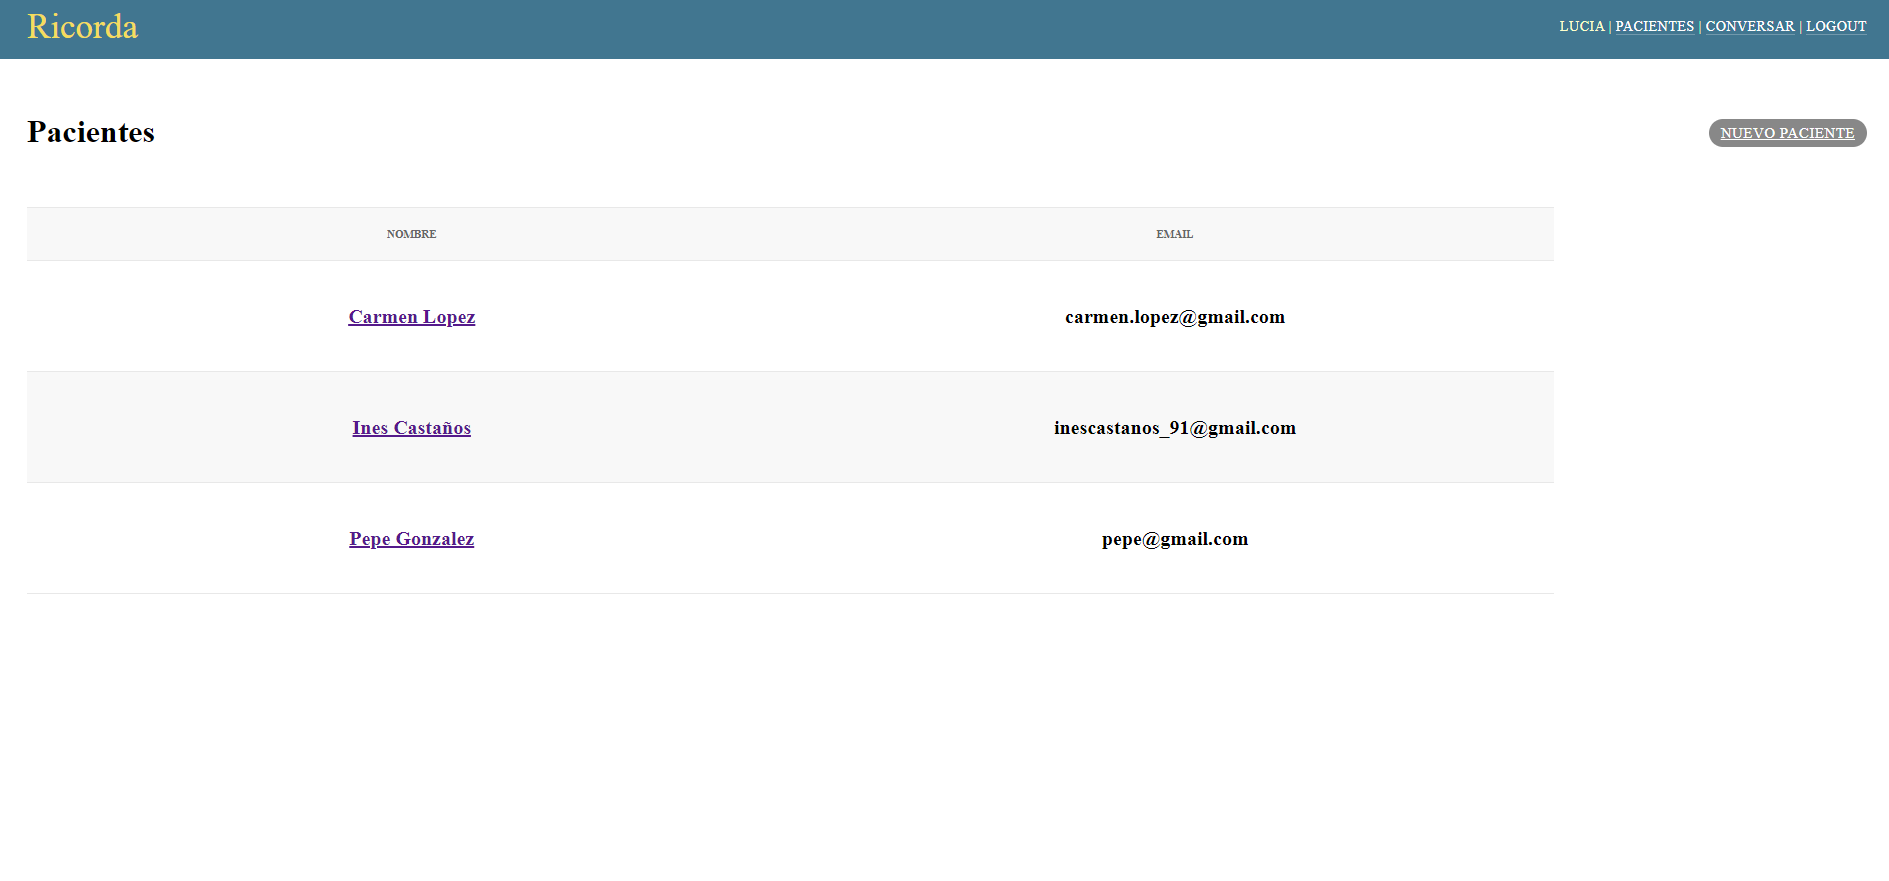
\includegraphics[scale=0.3]{Imagenes/Vectorial/funcionalidad_consultar_pacientes}
	\caption{Funcionalidad consultar pacientes registrados}
	\label{fig:funcionalidadconsultadepacientes}
\end{figure}

\subsection{Funcionalidad crear nuevo paciente}
\begin{figure}[h]
	\centering
	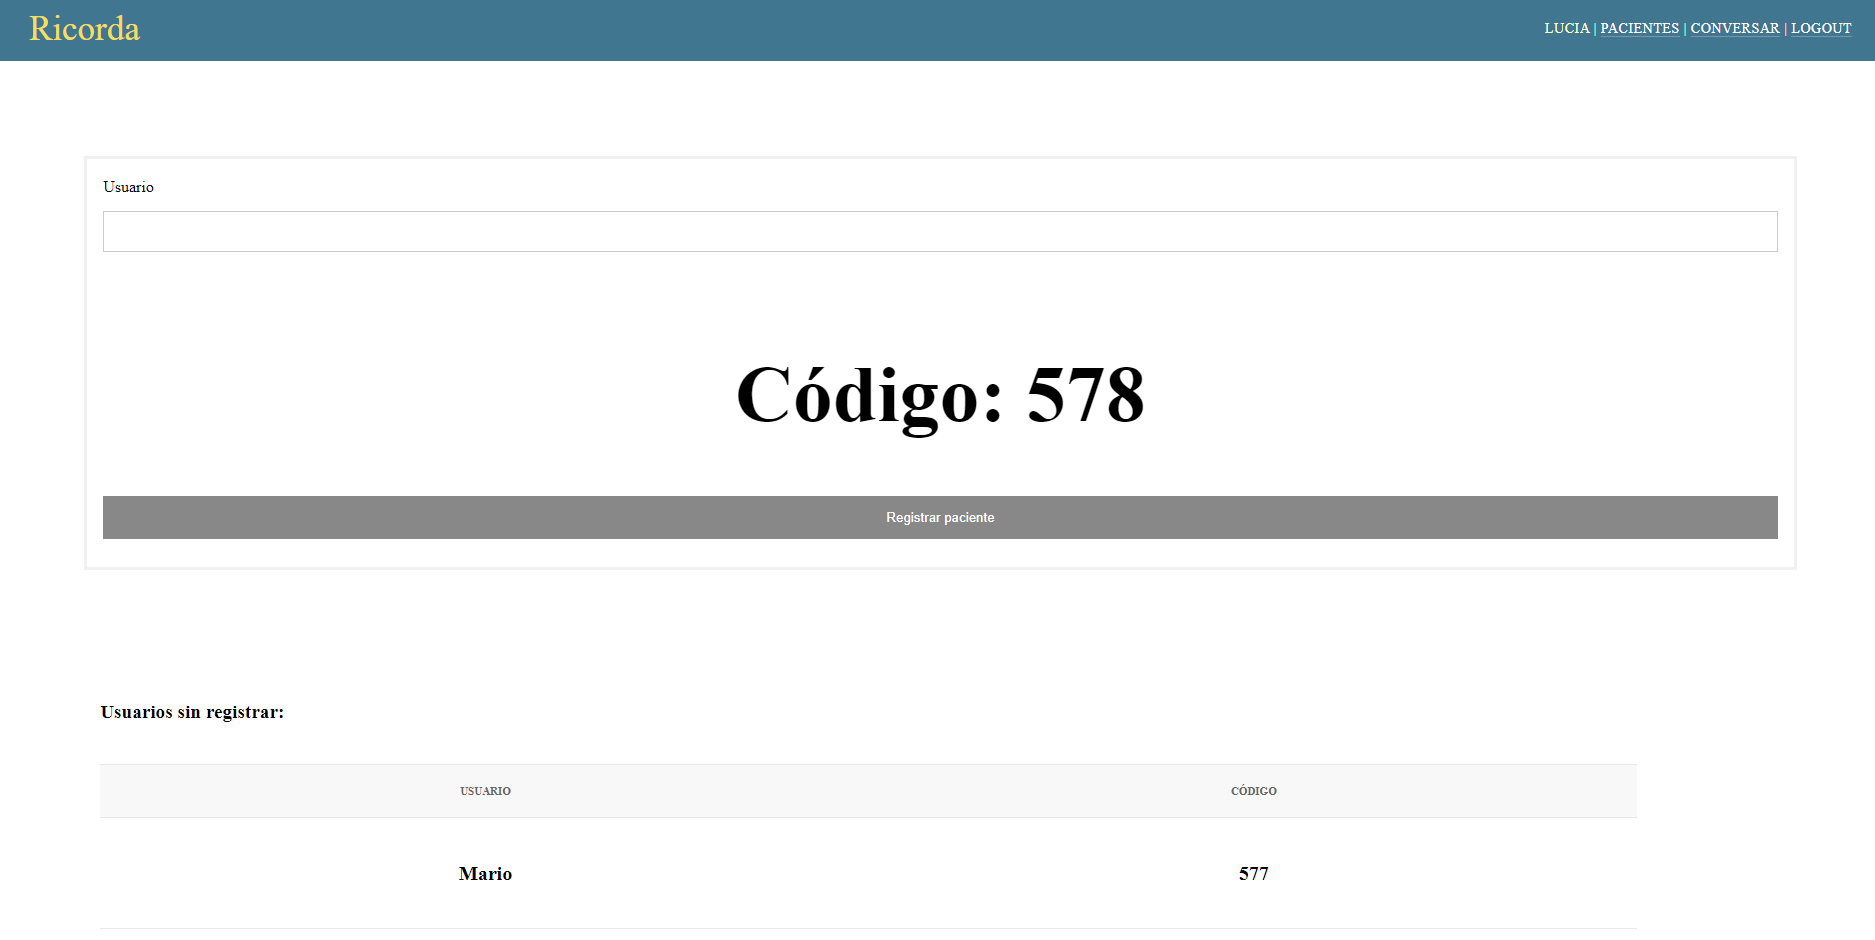
\includegraphics[scale=0.3]{Imagenes/Vectorial/funcionalidad_nuevo_paciente}
	\caption{Funcionalidad crear nuevo paciente}
	\label{fig:funcionalidadnuevopaciente}
\end{figure}

\subsection{Funcionalidad historia de vida de un paciente}
 

\begin{figure}[h]
	\centering
	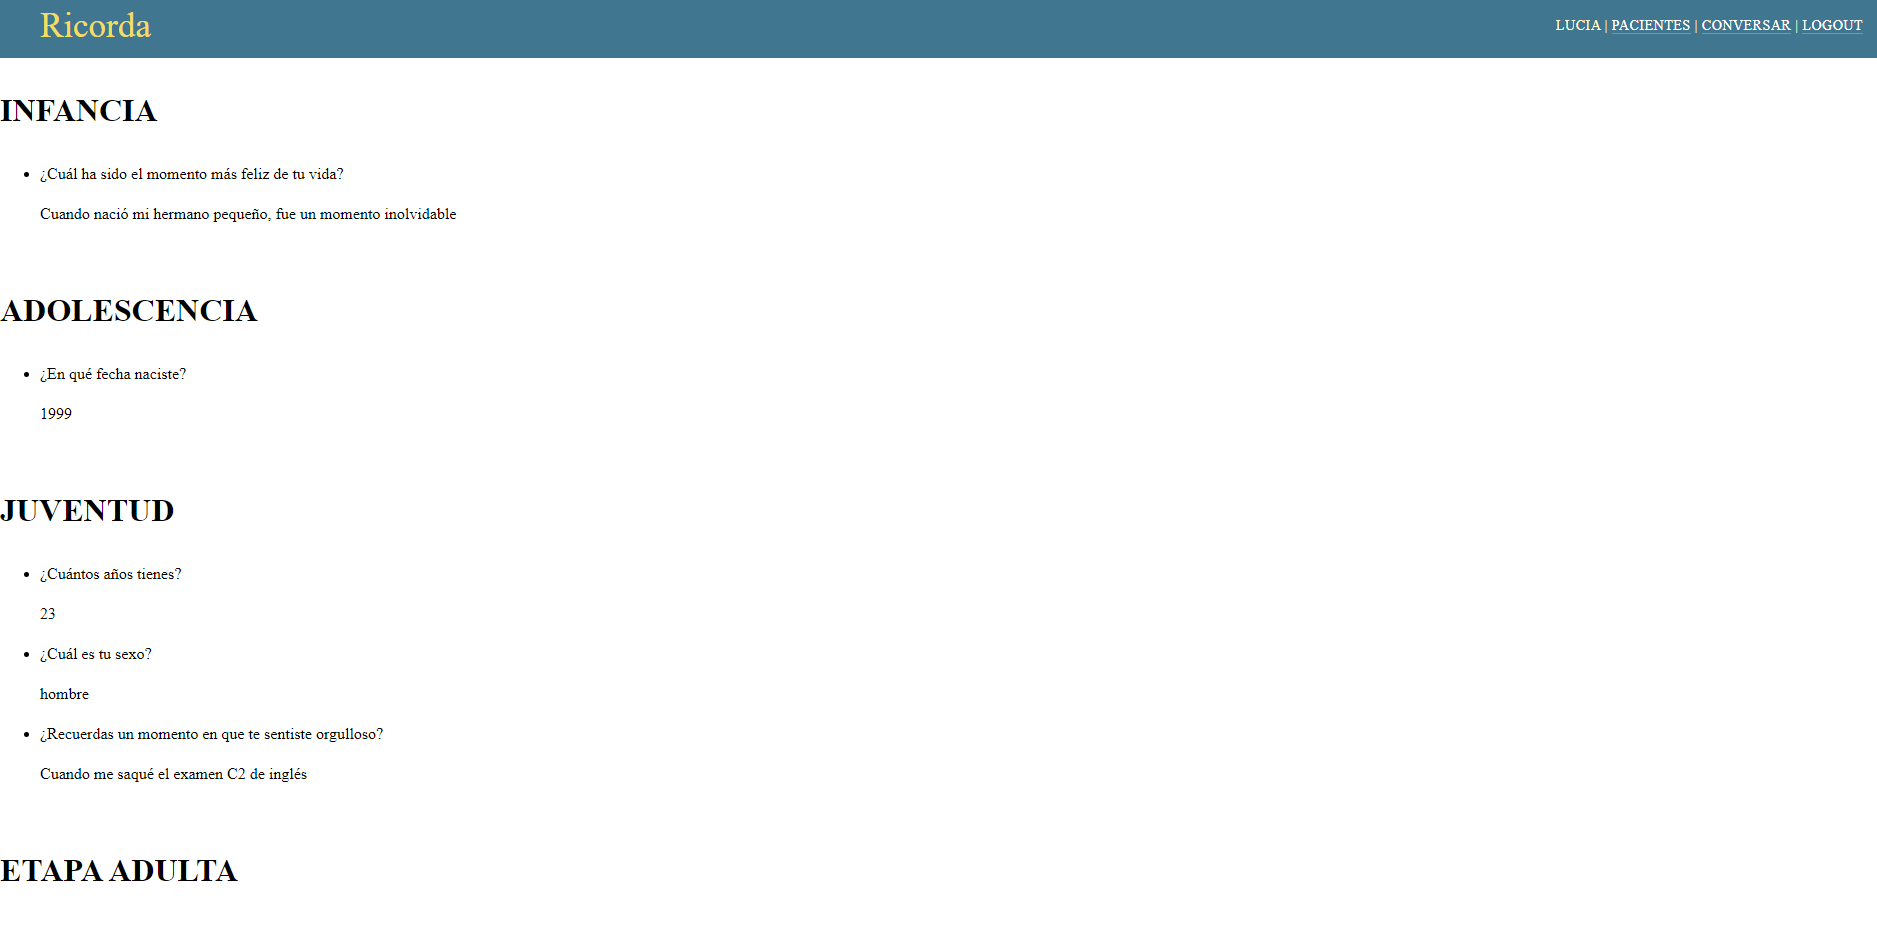
\includegraphics[scale=0.3]{Imagenes/Vectorial/funcionalidad_historia_vida}
	\caption{Funcionalidad crear nuevo paciente}
	\label{fig:funcionalidadhistoriavida}
\end{figure}




